% Latent Mamba: Adaptive Continuous Reasoning in Constant Memory
% Technical report. Single self-contained source: no external
% figures or .bib file. Compile with:  tectonic latent_mamba.tex
%                                  or:  pdflatex latent_mamba.tex (twice)
\documentclass[10pt]{article}

\usepackage[letterpaper,margin=1in]{geometry}
\usepackage[T1]{fontenc}
\usepackage{amsmath,amsthm}
\usepackage{newtxtext,newtxmath}
\usepackage{microtype}
\usepackage{booktabs}
\usepackage{multirow}
\usepackage{xcolor}
\usepackage{enumitem}
\usepackage{caption}
\usepackage{algorithm}
\usepackage{algpseudocode}
\usepackage{tikz}
\usetikzlibrary{arrows.meta,positioning,fit,calc,shapes.geometric,backgrounds}
\usepackage{pgfplots}
\pgfplotsset{compat=1.18}
\usepackage[colorlinks=true,linkcolor=blue!50!black,citecolor=blue!50!black,urlcolor=blue!50!black]{hyperref}

\captionsetup{font=small,labelfont=bf}

% Footer on every page (including the title page): repository link and page number.
\usepackage{fancyhdr}
\newcommand{\repourl}{https://github.com/The-Swarm-Corporation/latent-mamba}
\fancypagestyle{plain}{%
  \fancyhf{}%
  \renewcommand{\headrulewidth}{0pt}%
  \renewcommand{\footrulewidth}{0pt}%
  \fancyfoot[L]{\small GitHub: \href{\repourl}{\texttt{github.com/The-Swarm-Corporation/latent-mamba}}}%
  \fancyfoot[R]{\small\thepage}%
}
\pagestyle{plain}
\setlist{nosep,leftmargin=1.4em}
% Block paragraphs: no first-line indent, a small gap between paragraphs.
\setlength{\parindent}{0pt}
\setlength{\parskip}{0.55em plus 0.1em minus 0.1em}
% Run-in \paragraph headings: no extra space beyond the normal paragraph gap.
\makeatletter
\renewcommand\paragraph{\@startsection{paragraph}{4}{\z@}{0.01em}{-1em}{\normalfont\normalsize\bfseries}}
\makeatother

\definecolor{mambapurple}{RGB}{110,90,190}
\definecolor{addteal}{RGB}{40,150,140}
\definecolor{lossred}{RGB}{190,50,50}
\definecolor{softgray}{RGB}{120,120,120}

\newtheorem{proposition}{Proposition}
\newcommand{\eot}{\texttt{<eot>}}
\renewcommand{\bot}{\texttt{<bot>}}

\title{\textbf{Latent Mamba: Adaptive Continuous Reasoning in Constant Memory}}
\author{Kye Gomez\\Swarms Corp\\\texttt{kye@swarms.world}}
\date{November 9, 2026}

\begin{document}
\maketitle

\begin{abstract}
Chain-of-thought reasoning spends extra compute by writing tokens, and in a Transformer every token also grows the key--value cache. We describe \emph{Latent Mamba}, an architecture that lets a Mamba-2 language model reason in continuous latent space for an input-dependent number of steps while its memory stays constant. The model feeds its normalised final hidden state back as its next input through a learned \emph{thought projector} that adds a thinking-mode embedding, and a \emph{halting head} decides when to stop. We observe that in a selective state-space model, depth recurrence with a shared state is the same computation as interleaving self-generated latent inputs along the sequence, which motivates placing thoughts in time rather than in depth. Training follows a Coconut-style curriculum and then a PonderNet objective; because the recurrent state has a fixed size, the answer can be scored after every thought step in a single batched pass. Fine-tuning a pretrained 130M-parameter Mamba-2 on ProsQA with this recipe, the model answers \textbf{99.0\%} of held-out test questions while reasoning entirely in latent space with six thoughts, against 70.8\% for the same model trained to write its chain of thought and 74.6\% for the same model trained to answer directly. Replacing the thoughts with zeros or noise at test time drops accuracy to 77\% or below, so the gain comes from what the thoughts contain. The learned halting head stops after 3.1 thoughts on average at 98.6\% accuracy, matching a fixed budget of three, but adapts only weakly to problem difficulty. Measured on GPU, the recurrent state stays at 18.2\,MiB for budgets up to 4{,}096 thoughts, while our reference implementation is 3--5$\times$ slower per thought than GPT-2. All results come from one seed on one synthetic task.
\end{abstract}

% =========================================================================
\section{Introduction}
% =========================================================================

Language models solve multi-step problems better when they can compute before answering, usually by emitting a chain of thought (CoT) or a scratchpad~\cite{wei2022cot,nye2021scratchpad,kojima2022zeroshot}. This has two costs. Natural-language tokens are a narrow channel for intermediate state, and many of them serve fluency rather than reasoning~\cite{hao2024coconut}. In a Transformer~\cite{vaswani2017attention}, every generated token also adds an entry to the key--value (KV) cache, so memory grows with the length of the reasoning.

\emph{Latent reasoning} moves the intermediate computation into the model's continuous hidden space~\cite{zhu2025survey}. Coconut feeds the last hidden state back as the next input embedding instead of decoding it~\cite{hao2024coconut}. Recurrent-depth models iterate a shared block a variable number of times per token~\cite{geiping2025recurrent}. Both let a model think without writing text, but in a Transformer each continuous thought still occupies a cache slot.

Selective state-space models (SSMs)~\cite{gu2022s4} such as Mamba and Mamba-2~\cite{gu2023mamba,dao2024ssd} carry context in a fixed-size recurrent state instead of a cache, so a thought step costs constant memory: it updates the state and nothing else. We develop this into a concrete architecture, a training procedure, an implementation that trains from pretrained checkpoints, and a first evaluation.

\paragraph{Contributions.}
\begin{itemize}
\item A \emph{time--depth collapse} for SSMs (Proposition~\ref{prop:collapse}): depth recurrence with a shared state equals self-generated inputs interleaved along the sequence. Placing thoughts in time avoids the missing-state problem that per-iteration states create under adaptive exit.
\item \textbf{Latent Mamba} (Figure~\ref{fig:arch}): a thought projector with a thinking-mode embedding, a halting head, and functional fixed-size state handling. The added parameters are about 0.3\% of a 2.7B model and 0.6\% of a 130M model.
\item A training recipe (Algorithms~\ref{alg:curriculum} and~\ref{alg:ponder}) and an adaptive inference procedure (Algorithm~\ref{alg:generate}). PonderNet scoring is batched across thought steps, which is cheap only because SSM state is fixed-size.
\item Exact batching of prompts of different lengths (Proposition~\ref{prop:padding}) and a training path that cuts saved activations at batch 32 from 75\,GiB to 4.2\,GiB with identical gradients (Section~\ref{sec:scale}).
\item A reference implementation that loads pretrained Mamba-2 checkpoints without renaming, numerical verification of its kernels (Table~\ref{tab:verify}), and an experiment on ProsQA (Section~\ref{sec:experiments}) where the fully latent model reaches 99.0\% test accuracy against 70.8\% (written CoT) and 74.6\% (no CoT), with thought ablations, a thinking-budget sweep, learned halting, and measured memory and latency.
\end{itemize}

% =========================================================================
\section{Background}
% =========================================================================

\paragraph{Mamba-2.} Each layer projects its input $u_t$ to a gate $z_t$, a branch $(x_t, b_t, c_t)$ that passes through a causal depthwise convolution of width $K$, and per-head step sizes $\Delta_t = \operatorname{softplus}(w^\top u_t + \beta) > 0$. For head $h$ with decay rate $a_h < 0$, head input $x_t \in \mathbb{R}^P$ and $b_t, c_t \in \mathbb{R}^N$,
\begin{equation}
S_t = e^{\Delta_t a_h} S_{t-1} + \Delta_t\, x_t b_t^\top, \qquad y_t = S_t c_t + D_h x_t,
\label{eq:ssm}
\end{equation}
followed by a gated RMSNorm~\cite{zhang2019rmsnorm} and an output projection~\cite{dao2024ssd}. The recurrent state of a layer is the convolution window (the last $K{-}1$ inputs) together with $S \in \mathbb{R}^{H\times P\times N}$. Training processes whole sequences with the chunked SSD algorithm, a blocked form of a parallel scan~\cite{blelloch1990prefix,martin2018parallelizing}; inference applies Equation~\eqref{eq:ssm} one token at a time. Both compute the same function.

\paragraph{Continuous thought.} Coconut~\cite{hao2024coconut} marks a latent span with \bot{} and \eot. Inside the span the final hidden state is fed back as the next input embedding. It is trained with a curriculum adapted from implicit CoT~\cite{deng2024icot}: at stage $k$, the first $k$ language reasoning steps are replaced by $ck$ continuous thoughts, and the loss covers only the remaining text.

\paragraph{Adaptive computation.} ACT~\cite{graves2016act} and PonderNet~\cite{banino2021pondernet} let a network choose how many steps to run. PonderNet predicts, at each step $n$, a conditional halting probability $\lambda_n$. This gives the distribution $p_n = \lambda_n \prod_{j<n} (1 - \lambda_j)$. Training minimises $\sum_n p_n \mathcal{L}_n + \beta\, \mathrm{KL}(p \,\|\, \mathrm{Geo}(\lambda_p))$, where $\mathcal{L}_n$ is the task loss after step $n$.

% =========================================================================
\section{Latent Mamba}
% =========================================================================

\subsection{Where should a recurrent model think?}

A model can add computation along two axes~\cite{zhu2025survey,aviss2026sst}: \emph{depth} (iterate a block several times at one position) and \emph{time} (insert extra positions). Recurrent-depth Transformers take the depth route~\cite{geiping2025recurrent}. In an SSM the depth route raises a question that attention does not: which recurrent state does iteration $i$ at position $t$ read?

If each iteration has its own state stream, adaptive exit breaks the streams (Figure~\ref{fig:collapse}a). When token $t$ stops after one iteration, iterations two and up at token $t{+}1$ have no state from position $t$ to read. If instead all iterations share one state, the problem disappears and the computation becomes recurrence in time.

\begin{figure}[t]
\centering
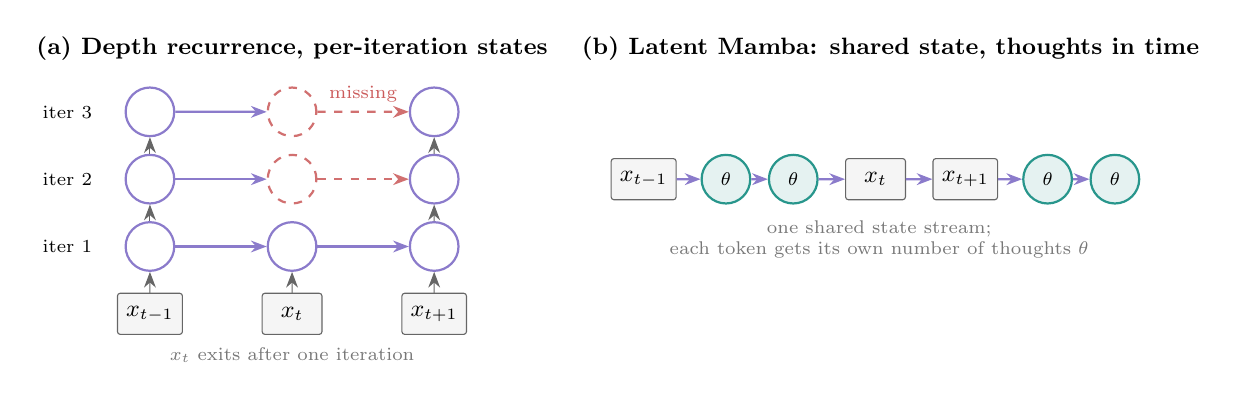
\begin{tikzpicture}[
  st/.style={circle,draw=mambapurple!80,thick,minimum size=6.5mm,inner sep=0pt},
  miss/.style={circle,draw=lossred!70,dashed,thick,minimum size=6.5mm,inner sep=0pt},
  tok/.style={rectangle,draw=black!60,fill=black!4,rounded corners=1pt,minimum width=8mm,minimum height=5.5mm,font=\small},
  flow/.style={-{Stealth[length=2mm]},thick,mambapurple!80},
  up/.style={-{Stealth[length=2mm]},black!60},
  scale=0.95,transform shape]
  % (a) depth recurrence
  \node[font=\small\bfseries] at (2.4,3.55) {(a) Depth recurrence, per-iteration states};
  \foreach \i/\y in {1/0.9,2/1.8,3/2.7}{
    \node[font=\scriptsize,anchor=east] at (-0.15,\y) {iter \i};
  }
  \foreach \x/\l in {0.5/{x_{t-1}},2.4/{x_t},4.3/{x_{t+1}}}{
    \node[tok] at (\x,0) {$\l$};
  }
  \node[st] (a1) at (0.5,0.9) {}; \node[st] (a2) at (0.5,1.8) {}; \node[st] (a3) at (0.5,2.7) {};
  \node[st] (b1) at (2.4,0.9) {}; \node[miss] (b2) at (2.4,1.8) {}; \node[miss] (b3) at (2.4,2.7) {};
  \node[st] (c1) at (4.3,0.9) {}; \node[st] (c2) at (4.3,1.8) {}; \node[st] (c3) at (4.3,2.7) {};
  \draw[flow] (a1) -- (b1); \draw[flow] (b1) -- (c1);
  \draw[flow] (a2) -- (b2); \draw[flow] (a3) -- (b3);
  \draw[-{Stealth[length=2mm]},thick,lossred!70,dashed] (b2) -- (c2);
  \draw[-{Stealth[length=2mm]},thick,lossred!70,dashed] (b3) -- node[above,font=\scriptsize,text=lossred!80] {missing} (c3);
  \foreach \c in {a,c}{ \draw[up] (\c1) -- (\c2); \draw[up] (\c2) -- (\c3); }
  \draw[up] (0.5,0.28) -- (a1); \draw[up] (2.4,0.28) -- (b1); \draw[up] (4.3,0.28) -- (c1);
  \node[font=\scriptsize,text=softgray] at (2.4,-0.55) {$x_t$ exits after one iteration};
  % (b) latent mamba
  \begin{scope}[xshift=7.1cm]
  \node[font=\small\bfseries] at (3.3,3.55) {(b) Latent Mamba: shared state, thoughts in time};
  \node[tok] (s1) at (0,1.8) {$x_{t-1}$};
  \node[st,fill=addteal!12,draw=addteal] (s2) at (1.1,1.8) {\scriptsize$\theta$};
  \node[st,fill=addteal!12,draw=addteal] (s3) at (2.0,1.8) {\scriptsize$\theta$};
  \node[tok] (s4) at (3.1,1.8) {$x_t$};
  \node[tok] (s5) at (4.3,1.8) {$x_{t+1}$};
  \node[st,fill=addteal!12,draw=addteal] (s6) at (5.4,1.8) {\scriptsize$\theta$};
  \node[st,fill=addteal!12,draw=addteal] (s7) at (6.3,1.8) {\scriptsize$\theta$};
  \foreach \a/\b in {s1/s2,s2/s3,s3/s4,s4/s5,s5/s6,s6/s7}{ \draw[flow] (\a) -- (\b); }
  \node[font=\scriptsize,text=softgray,align=center] at (3.15,1.0) {one shared state stream;\\each token gets its own number of thoughts $\theta$};
  \end{scope}
\end{tikzpicture}
\caption{(a) Per-iteration state streams break under adaptive exit: when $x_t$ halts after one iteration, the deeper iterations at $x_{t+1}$ have no state to read. (b) With a shared state, depth recurrence becomes thoughts interleaved in time (Proposition~\ref{prop:collapse}). Purple arrows carry SSM state.}
\label{fig:collapse}
\end{figure}

\begin{proposition}[Time--depth collapse]\label{prop:collapse}
Let $F : (u, S) \mapsto (h, S')$ be one pass of an SSM stack over a single input, and let $g$ map outputs to inputs. Suppose the model runs $r_t$ iterations at position $t$. Iteration $i{+}1$ takes input $g(h_t^{(i)})$ and the state $S_t^{(i)}$ left by iteration $i$; iteration 1 at position $t{+}1$ takes $u_{t+1}$ and $S_t^{(r_t)}$. Then every output and state equals that of a single pass of $F$ over the interleaved sequence $\big(u_1, g(h_1^{(1)}), \dots, g(h_1^{(r_1-1)}), u_2, \dots\big)$.
\end{proposition}
\begin{proof}[Proof sketch]
Both procedures apply $F$ to the same (input, state) pairs in the same order. Induct on the position in the interleaved sequence.
\end{proof}

The statement is elementary, but it fixes the design. In an SSM, shared-state depth recurrence \emph{is} thinking in time. That form keeps memory constant, needs no new kernels, and has no missing-state problem, so Latent Mamba places its thoughts along the sequence (Figure~\ref{fig:collapse}b). The feedback map $g$ is the thought projector.

\subsection{Architecture}

\begin{figure}[t]
\centering
\resizebox{\linewidth}{!}{%
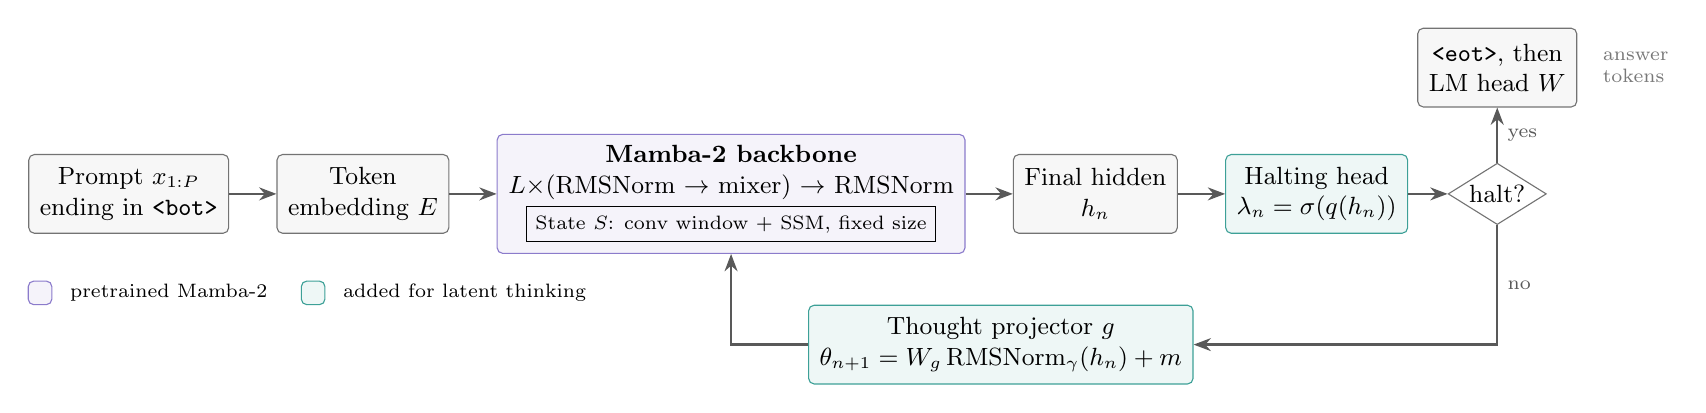
\begin{tikzpicture}[
  box/.style={rectangle,draw=black!55,fill=black!3,rounded corners=2pt,align=center,font=\small,minimum height=10mm,inner sep=4pt},
  pre/.style={box,draw=mambapurple!80,fill=mambapurple!7},
  add/.style={box,draw=addteal!90,fill=addteal!8},
  arr/.style={-{Stealth[length=2.2mm]},thick,black!65},
  node distance=6mm]
  \node[box] (prompt) {Prompt $x_{1:P}$\\ending in \bot};
  \node[box,right=of prompt] (emb) {Token\\embedding $E$};
  \node[pre,right=of emb,minimum width=3.6cm] (bb) {\textbf{Mamba-2 backbone}\\$L\times$(RMSNorm $\to$ mixer) $\to$ RMSNorm\\[2pt]\fbox{\scriptsize State $S$: conv window + SSM, fixed size}};
  \node[box,right=of bb] (h) {Final hidden\\$h_n$};
  \node[add,right=of h] (halt) {Halting head\\$\lambda_n=\sigma(q(h_n))$};
  \node[diamond,draw=black!55,aspect=1.6,inner sep=1pt,font=\small,right=5mm of halt] (dec) {halt?};
  \node[box,above=7mm of dec] (out) {\eot, then\\LM head $W$};
  \node[font=\scriptsize,text=softgray,right=2mm of out,align=left] {answer\\tokens};
  \node[add,below=9mm of h,xshift=-12mm] (proj) {Thought projector $g$\\$\theta_{n+1} = W_g\,\mathrm{RMSNorm}_\gamma(h_n) + m$};
  \draw[arr] (prompt) -- (emb); \draw[arr] (emb) -- (bb); \draw[arr] (bb) -- (h); \draw[arr] (h) -- (halt); \draw[arr] (halt) -- (dec);
  \draw[arr] (dec) -- node[right,font=\scriptsize] {yes} (out);
  \draw[arr] (dec.south) |- node[pos=0.25,right,font=\scriptsize] {no} (proj.east);
  \draw[arr] (proj.west) -| (bb.south);
  \node[pre,minimum height=3mm,minimum width=3mm,inner sep=0pt] (l1) at ($(prompt.south west)+(0.15,-0.75)$) {};
  \node[font=\scriptsize,right=1mm of l1] (l1t) {pretrained Mamba-2};
  \node[add,minimum height=3mm,minimum width=3mm,inner sep=0pt,right=3mm of l1t] (l2) {};
  \node[font=\scriptsize,right=1mm of l2] {added for latent thinking};
\end{tikzpicture}%
}
\caption{Latent Mamba. The prompt is prefilled with the parallel scan. Each thought feeds the projected final hidden state back as the next input and updates only the fixed-size state $S$. The halting head decides between another thought and decoding the answer after \eot.}
\label{fig:arch}
\end{figure}

The prompt ends in \bot. Let $h_0$ be the final normalised hidden state at \bot, $S_0$ the state after the prompt, and $F$ one recurrent step of the whole backbone. Thought step $n \ge 1$ computes
\begin{align}
\theta_n &= W_g\, \mathrm{RMSNorm}_\gamma(h_{n-1}) + m, \label{eq:proj}\\
(h_n, S_n) &= F(\theta_n, S_{n-1}), \qquad \lambda_n = \sigma\big(q(h_n)\big). \label{eq:step}
\end{align}
After halting, the model reads \eot{} and decodes the answer with the language-model head $W$. Table~\ref{tab:params} lists the added parameters.

\paragraph{Thought projector.} The final hidden state lives in output space, not input-embedding space. Mamba computes $\Delta_t$, $b_t$ and $c_t$ from its input, so off-distribution inputs push these projections into regimes never seen in training. We therefore initialise $W_g = I$, $m = 0$ and $\gamma$ to the RMS of the embedding matrix. At initialisation, the model is exactly Coconut with thoughts at the scale of a token embedding.

\paragraph{Thinking-mode embedding and prompt retention.} By Equation~\eqref{eq:ssm}, after $n$ thoughts the part of head $h$'s state that came from the prompt has been multiplied by
\begin{equation}
\textstyle\prod_{k=1}^{n} e^{\Delta_{h,k} a_h} \;=\; \exp\!\big(a_h \sum_{k=1}^{n} \Delta_{h,k}\big).
\label{eq:decay}
\end{equation}
Long thinking can thus erase the question. $\Delta_{h,k}$ is a function of the input, so the learned vector $m$ gives the model a direct way to select small step sizes while thinking. This retains the prompt, while thought content still enters through the convolution and the $x$ and $b$ paths. The cumulative step size $\sum_k \Delta_{h,k}$ is a cheap diagnostic of prompt decay.

\paragraph{Halting head.} $q$ is a two-layer MLP. Its last layer has zero weights and bias $\operatorname{logit}(\lambda_p)$, so the initial halting distribution equals the geometric prior and the initial KL term is zero.

\paragraph{Why thoughts add expressivity.} Within one pass, each layer's state update in Equation~\eqref{eq:ssm} is linear in $S$. A thought composes the full nonlinear network, including gates, normalisation and all layers, before the next state update. So $n$ thoughts form a nonlinear recurrence of depth $n\cdot L$ in latent space, applied to whatever the state already holds.

\begin{table}[t]
\centering
\small
\begin{tabular}{@{}lcrrrr@{}}
\toprule
& & \multicolumn{2}{c}{2.7B ($d{=}2560$)} & \multicolumn{2}{c}{130M ($d{=}768$)} \\
\cmidrule(lr){3-4}\cmidrule(l){5-6}
Module & Params & Count & Share & Count & Share \\
\midrule
Thought projector & $d^2 + 2d$ & 6.56M & 0.24\% & 0.59M & 0.46\% \\
Halting head & $\tfrac{d^2}{4} + \tfrac{d}{2} + 1$ & 1.64M & 0.06\% & 0.15M & 0.11\% \\
\midrule
Total & & 8.20M & 0.30\% & 0.74M & 0.57\% \\
\bottomrule
\end{tabular}
\caption{Parameters added to Mamba-2 models.}
\label{tab:params}
\end{table}

\subsection{Memory}

The state of the whole model occupies
\begin{equation}
L\,\big[(K-1)(d_{\text{inner}} + 2N) + HPN\big]
\label{eq:mem}
\end{equation}
values, independent of both prompt length and thought count. For the Mamba-2 2.7B configuration ($L{=}64$, $d{=}2560$, $N{=}128$, $P{=}64$, $K{=}4$) this is 671{,}488 values per layer, or 82.0\,MiB in fp16. A 32-layer Transformer of the same width with multi-head attention stores 0.3125\,MiB of KV cache per token; with $4\times$ grouped-query attention~\cite{ainslie2023gqa}, 0.078\,MiB. Multi-query attention~\cite{shazeer2019mqa} shrinks the per-token cost further, but the cache still grows with every token.

Figure~\ref{fig:memory} compares the three after a 512-token prompt. The grouped-query Transformer is smaller until about 1{,}050 cached tokens, so the advantage is not universal. Beyond that point every Transformer thought costs memory, while Latent Mamba's footprint stays flat at any thinking budget. At the scale used in our experiments the comparison is starker: Mamba-2 130M ($L{=}24$, $d_{\text{inner}}{=}1536$, $H{=}24$) holds 9.25\,MiB of state in bf16, while GPT-2 124M~\cite{radford2019gpt2} stores 36\,KiB of KV cache per token, so its cache already exceeds Latent Mamba's whole state after 263 tokens. Section~\ref{sec:bench} measures both on GPU.

\begin{figure}[t]
\centering
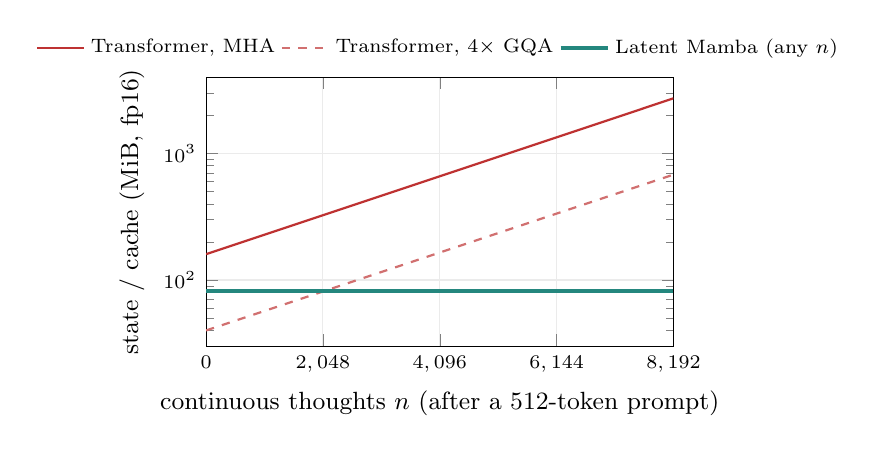
\begin{tikzpicture}
\begin{axis}[
  width=0.62\linewidth, height=5.0cm,
  xmin=0, xmax=8192, ymode=log, ymin=30, ymax=4000,
  xlabel={continuous thoughts $n$ (after a 512-token prompt)},
  ylabel={state / cache (MiB, fp16)},
  xtick={0,2048,4096,6144,8192},
  scaled x ticks=false,
  xticklabel style={/pgf/number format/1000 sep={,}},
  legend style={font=\scriptsize,at={(0.5,1.03)},anchor=south,legend columns=3,draw=none},
  tick label style={font=\scriptsize}, label style={font=\small},
  grid=major, grid style={black!8}]
\addplot[lossred,thick,domain=0:8192,samples=2] {(512+x)*0.3125};
\addplot[lossred!70,thick,dashed,domain=0:8192,samples=2] {(512+x)*0.078125};
\addplot[addteal!90!black,very thick,domain=0:8192,samples=2] {82.0};
\legend{{Transformer, MHA},{Transformer, $4\times$ GQA},{Latent Mamba (any $n$)}}
\end{axis}
\end{tikzpicture}
\caption{Analytic memory for a 2.7B-scale configuration at batch size 1. Transformer KV cache grows with every thought; the Latent Mamba state does not.}
\label{fig:memory}
\end{figure}

\subsection{Exact batching of prompts with different lengths}

Real prompts differ in length. Padding them on the left would normally push pad tokens through the recurrent state. We avoid this with a mask that makes pad positions an exact identity on the state.

\begin{proposition}[Exact left padding]\label{prop:padding}
Run a Mamba-2 layer from the zero state over a left-padded sequence. At every padded position, set the convolution input $(x_t, b_t, c_t)$ to zero before the convolution, and set $\Delta_t = 0$ after the softplus. Then the hidden states at real positions, and the final conv window and SSM state, equal those of the unpadded sequence. The same holds for the whole stack, applying the mask in every layer.
\end{proposition}
\begin{proof}[Proof sketch]
With $\Delta_t = 0$, Equation~\eqref{eq:ssm} gives $S_t = S_{t-1}$, so the SSM state stays zero through the padding. The convolution window after the padding contains only zeros, which equals the zero initial window. Real positions therefore see exactly the state and window they would see without padding. Outputs at padded positions are arbitrary but never read: every later layer masks them again.
\end{proof}

Proposition~\ref{prop:padding} lets a batch mix prompts of any lengths with no bucketing. The implementation verifies it in float64 (Table~\ref{tab:verify}).

% =========================================================================
\section{Training and inference}
% =========================================================================

\begin{algorithm}[t]
\caption{Curriculum loss with per-example thought counts}
\label{alg:curriculum}
\begin{algorithmic}[1]
\Require prompts $x_{1:P}$ ending in \bot{} (left padded, with mask); targets $y_{1:T}$; counts $n_b$
\State $(H, S) \gets \textsc{Backbone}(E(x), \mathbf{0})$ \Comment{chunked scan, masked}
\State $h \gets H_P$ \Comment{hidden state at \bot}
\For{$i = 1, \dots, \max_b n_b$}
  \State $(h', S') \gets F\big(W_g\,\mathrm{RMSNorm}(h) + m,\; S\big)$ \Comment{one step}
  \State $a_b \gets [\,i \le n_b\,]$ for every example $b$
  \State $h \gets a \odot h' + (1-a)\odot h$; \quad $S \gets a \odot S' + (1-a)\odot S$
\EndFor
\State $Z \gets \textsc{Backbone}\big(E([\eot, y_{1:T-1}]), S\big)$ \Comment{teacher forcing}
\State \Return $\mathrm{CE}(WZ, y)$ over non-padding targets
\end{algorithmic}
\end{algorithm}

\subsection{Curriculum}

We follow Coconut~\cite{hao2024coconut} (Algorithm~\ref{alg:curriculum}). Stage 0 is language CoT after \bot\eot, i.e.\ zero thoughts. At stage $k \le K$, the first $k$ of an example's $s$ reasoning steps are removed from the target and replaced by $ck$ thoughts; as in Coconut, the thought count is $ck$ even when $s < k$. A final stage $K{+}1$ removes every step and uses $cK$ thoughts. Thought counts can differ within a batch. An example that has finished thinking is frozen by selecting its old state and hidden vector, so one batch runs $\max_b n_b$ steps. Gradients flow through every thought. For long budgets, the state can be detached after a fixed number of steps, as in recurrent-depth training~\cite{geiping2025recurrent}. We reset the optimiser at each stage, as Coconut does, and keep the checkpoint with the best validation accuracy within each stage.

\begin{algorithm}[t]
\caption{PonderNet step with batched branch scoring}
\label{alg:ponder}
\begin{algorithmic}[1]
\Require prompts $x$ ending in \bot; targets $y$; budget $N$; prior $\lambda_p$; weight $\beta$
\State $(H, S) \gets \textsc{Backbone}(E(x), \mathbf{0})$; \quad $h \gets H_P$
\For{$n = 1, \dots, N$}
  \State $(h, S) \gets F\big(W_g\,\mathrm{RMSNorm}(h) + m,\; S\big)$
  \State $\lambda_n \gets \sigma(q(h))$; \quad $S^{(n)} \gets S$
\EndFor
\State $\lambda_N \gets 1$; \quad $p_n \gets \lambda_n \prod_{j<n}(1-\lambda_j)$ \Comment{log space}
\State $\bar S \gets \textsc{Concat}_{\text{batch}}(S^{(1)}, \dots, S^{(N)})$
\State $\ell_{1:N} \gets$ per-example CE of $y$ decoded from $\bar S$ \Comment{one pass}
\State $g_n \propto \lambda_p (1-\lambda_p)^{n-1}$, normalised on $\{1..N\}$
\State \Return $\sum_n p_n \ell_n + \beta \sum_n p_n \log(p_n / g_n)$
\end{algorithmic}
\end{algorithm}

\subsection{Learning to halt}

The final stage trains the halting head with the PonderNet objective (Algorithm~\ref{alg:ponder}). The model takes $N$ thoughts and keeps the state after each. Because these states have a fixed size, the $N$ branches can be concatenated along the batch axis, and the answer is scored from all of them in one pass of $N \cdot B$ short sequences. The extra cost is about $N$ answer passes. In a Transformer, the same branching would copy $N$ KV caches of growing length.

We set $\lambda_N = 1$ so that $p$ is a proper distribution, and use the geometric prior truncated to $\{1, \dots, N\}$. Two cheaper alternatives need no halting training: a zero-shot convergence rule, as used for recurrent-depth models~\cite{geiping2025recurrent,tur2026rdvla}, and reinforcement learning with a per-thought compute penalty.

\begin{algorithm}[t]
\caption{Adaptive latent generation}
\label{alg:generate}
\begin{algorithmic}[1]
\Require prompt $x$ ending in \bot; maximum $N$; threshold $\tau$
\State $(H, S) \gets \textsc{Backbone}(E(x), \mathbf{0})$; \quad $h \gets H_P$
\State $\rho \gets 1$; \quad $n \gets 0$ \Comment{$\rho$: probability of not halting}
\While{$n < N$}
  \State $(h, S) \gets F\big(W_g\,\mathrm{RMSNorm}(h) + m,\; S\big)$; \quad $n \gets n + 1$
  \State $\rho \gets \rho\,(1 - \sigma(q(h)))$
  \If{$1 - \rho \ge \tau$} \textbf{break} \EndIf
\EndWhile
\State $v \gets \eot$
\Repeat
  \State $(h, S) \gets F(E(v), S)$; \quad $v \gets \arg\max W h$; \quad emit $v$
\Until{end token or length limit}
\end{algorithmic}
\end{algorithm}

\subsection{Adaptive inference}

Algorithm~\ref{alg:generate} thinks until a halting rule fires and then decodes. The learned rule stops at the median of the predicted halting distribution, when $1 - \prod_j (1 - \lambda_j) \ge \tau$ with $\tau = 0.5$. The convergence rule stops when $\|h_n - h_{n-1}\| / \|h_{n-1}\| < \epsilon$. A fixed rule runs exactly $N$ thoughts, matching the curriculum stages. Within a batch, halted examples are frozen while the others continue, and memory is constant throughout.

\subsection{Training at scale}
\label{sec:scale}

Our first full-size run ran out of memory on a 93\,GiB GPU at batch 32. We measured the activations saved for the backward pass on the longest ProsQA prompts (592 tokens) and made two changes.

\paragraph{No per-head copies of $b$ and $c$.} Mamba-2 checkpoints use a single group, so $b_t$ and $c_t$ are shared by all heads. A direct transcription of the chunked SSD algorithm broadcasts them to every head before the contractions, which materialises $H$ copies (24 for the 130M model). We instead contract $c_l^\top b_s$ once per chunk and apply the per-head decay afterwards, and fold the per-head decay into $x$ before forming chunk states. This removes roughly 30\% of the saved bytes per token and leaves results unchanged (Table~\ref{tab:verify}).

\paragraph{Activation checkpointing.} We recompute each Mamba layer during the backward pass instead of storing its internals~\cite{chen2016checkpoint}. Because state updates are functional, a layer is a pure function of (input, state, mask) and checkpointing needs no special handling. Saved activations for a batch of 32 of the longest prompts fall from 75.0\,GiB to 4.2\,GiB. Loss and gradients are identical (maximum relative difference 0 in float32), at the cost of about one extra forward pass.

\paragraph{Precision.} We train under bf16 autocast~\cite{micikevicius2018mixed} but run the selective scan and the single-step recurrence in float32: the scan exponentiates cumulative sums of $\Delta a$, which bf16 represents poorly. An optional fused path uses the Triton kernels of \texttt{mamba\_ssm} for prompts and answers. It is checked against the reference scan, forward and backward, before use.

% =========================================================================
\section{Reference implementation}
% =========================================================================

The implementation is plain PyTorch with no custom kernels. Sequences use the chunked SSD algorithm~\cite{dao2024ssd} started from an arbitrary initial state; single tokens use the exact recurrence of Equation~\eqref{eq:ssm}. State updates are functional: they return new tensors, so a cache can be branched, frozen per example or concatenated without side effects, as Algorithms~\ref{alg:curriculum} and~\ref{alg:ponder} require. The file also contains a diagnostic ablation that replaces thought content with zeros, which turns thoughts into pause tokens~\cite{goyal2024pause}, or with noise of matching RMS.

\paragraph{Pretrained weights.} The mixer follows Mamba-2's parameterisation (input projection to $[z, x, b, c, \Delta]$, depthwise causal convolution over $(x, b, c)$, per-head $A$, $\Delta$ bias and $D$, gated RMSNorm), and the parameter names of the public \texttt{state-spaces/mamba2-*} checkpoints, pretrained on the Pile~\cite{gao2020pile}, already match ours, so they load without renaming; only the two new modules are initialised fresh. As a sanity check, the ported 130M model scores 2.63 nats per token on a held-out Wikipedia paragraph and continues ``The capital of France is'' fluently. The three special tokens (\bot, \eot, pad) use spare rows of the checkpoint's padded vocabulary and are initialised from the embedding of ``\texttt{<<}'', as Coconut does.

\paragraph{Verification.} The method depends on one property: continuing from a stored state must give exactly the result of an uninterrupted pass. Table~\ref{tab:verify} reports the checks, run in float64 on the current implementation. The scan uses three chunks with end padding and a random initial state.

\begin{table}[t]
\centering
\small
\begin{tabular}{@{}lr@{}}
\toprule
Check (float64) & Max.\ abs.\ error \\
\midrule
Chunked scan vs.\ recurrence, outputs (batch 3, length 21, $H{=}4$, $P{=}8$, $N{=}16$, chunk 8) & $1.1\times10^{-14}$ \\
Chunked scan vs.\ recurrence, final state & $2.7\times10^{-15}$ \\
Prefill + per-token continuation vs.\ one pass, logits & $2.2\times10^{-16}$ \\
\quad final state after continuation & $1.4\times10^{-17}$ \\
Left-padded vs.\ unpadded prompt, hidden state (Proposition~\ref{prop:padding}) & $2.2\times10^{-16}$ \\
\quad conv window and SSM state & $2.2\times10^{-16}$ \\
Halting distribution sums to one & $0$ \\
Activation checkpointing vs.\ none, gradients (float32, relative) & $0$ \\
\bottomrule
\end{tabular}
\caption{Numerical checks of the implementation. All but the last are part of the file's built-in self-test, which also checks that gradients reach the thought projector and the halting head, that a stopped example stays frozen while others continue, and that generation runs under every halting rule.}
\label{tab:verify}
\end{table}

% =========================================================================
\section{Experiments}
\label{sec:experiments}
% =========================================================================

\subsection{Setup}

\paragraph{Task.} ProsQA~\cite{hao2024coconut} asks whether an entity belongs to one of two fictional concepts, given a randomly generated graph of ``every A is a B'' facts. Answering requires finding a path through the graph, with distracting branches, so it rewards planning and search. Each question has two candidate answers, so chance is 50\%. We use Coconut's splits (17{,}886 / 300 / 500 examples). With the GPT-NeoX tokenizer~\cite{black2022neox}, questions are long (median 357 tokens, 99th percentile 502, maximum 591); the written reasoning plus answer is short (median 50 tokens). Questions need 3 to 6 gold reasoning steps (124, 133, 36 and 7 validation questions and 202, 217, 69 and 12 test questions respectively).

\paragraph{Models.} All three models start from the same pretrained Mamba-2 130M checkpoint and differ only in what they are trained to output:
\begin{itemize}
\item \textbf{No CoT:} question \bot\eot{} \texttt{\#\#\# answer}.
\item \textbf{Written CoT:} question \bot\eot{} step$_1$ \dots{} step$_s$ \texttt{\#\#\# answer}.
\item \textbf{Latent Mamba:} the full curriculum (stage 0 = written CoT, stages 1--6, final stage with all steps replaced by thoughts), then the halting stage.
\end{itemize}

\paragraph{Training.} We follow Coconut's published ProsQA configuration: $c = 1$ thought per step, $K = 6$ latent stages, 5 epochs per stage including stage 0, and 15 epochs in the final stage, for 50 epochs in total; the halting stage adds 5 epochs. The baselines train for 5 epochs, matching stage 0. Table~\ref{tab:hparams} lists the remaining settings. One difference from Coconut is the batch: we train on one GPU with batch 32, where Coconut used four GPUs with 32 each. Each phase continues from the weights at the end of the previous one, and the checkpoint kept for a phase is its best validation epoch, as in Coconut. Answers are decoded greedily (up to 128 tokens) and scored by exact match of the text after the last ``\texttt{\#}'', Coconut's rule.

\paragraph{Evaluation.} We report test accuracy on the 500 held-out questions for the kept checkpoint of each model; for Latent Mamba this is the halting-stage checkpoint (epoch 51). We run it in six modes: \emph{learned} halting ($\tau = 0.5$, at most $N = 6$ thoughts); \emph{fixed}, exactly 6 thoughts; \emph{convergence} halting (relative change below $10^{-2}$, at most 6); \emph{no thoughts}, decoding directly after \bot\eot; and two ablations that run 6 thoughts but replace the content of every thought with zeros or with noise of matching RMS. A sweep fixes the budget at every value from 0 to 12 thoughts.

\begin{table}[t]
\centering
\small
\begin{tabular}{@{}ll@{\qquad}ll@{}}
\toprule
Base model & \texttt{state-spaces/mamba2-130m} & Optimiser & AdamW~\cite{loshchilov2019adamw}, lr $10^{-4}$ (constant), wd 0.01 \\
Hardware & $1\times$ H100 NVL (94\,GB) & Batch & 32, gradient clipping 1.0 \\
Precision & bf16 autocast, float32 scan & Optimiser reset & every stage \\
Chunk length & 64 & Checkpoint & best validation accuracy per stage \\
Thoughts per step $c$ & 1 & Halting & $N = 6$, $\lambda_p = 0.2$, $\beta = 0.01$ \\
Latent stages $K$ & 6 & Seed & 0 (one run per model) \\
\bottomrule
\end{tabular}
\caption{Training settings for the ProsQA experiments.}
\label{tab:hparams}
\end{table}

\subsection{Results}

\begin{figure}[t]
\centering
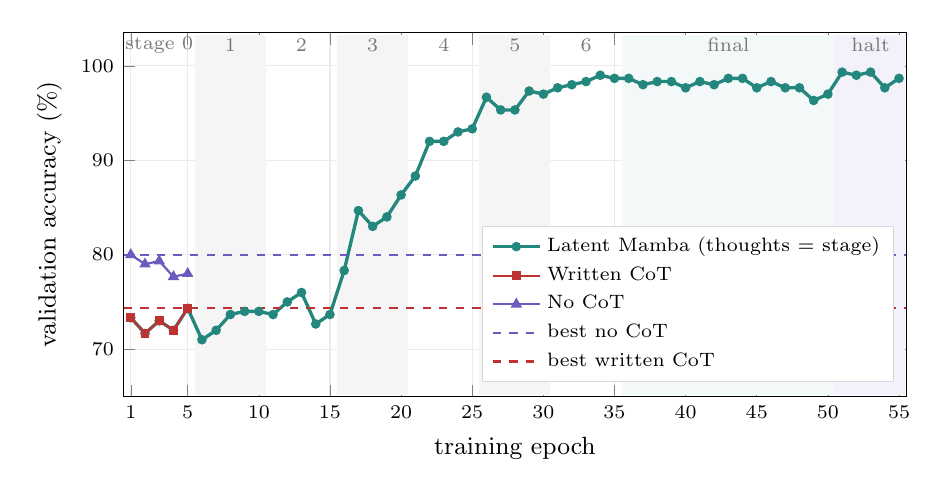
\begin{tikzpicture}
\begin{axis}[
  width=0.95\linewidth, height=6.2cm,
  xmin=0.5, xmax=55.5, ymin=65, ymax=103.5,
  xlabel={training epoch}, ylabel={validation accuracy (\%)},
  xtick={1,5,10,15,20,25,30,35,40,45,50,55},
  legend style={font=\scriptsize,at={(0.985,0.04)},anchor=south east,draw=black!15,fill=white,cells={anchor=west}},
  tick label style={font=\scriptsize}, label style={font=\small},
  grid=major, grid style={black!8}, clip=false]
  % stage shading and labels
  \fill[black!4] (axis cs:5.5,65.2) rectangle (axis cs:10.5,103.3);
  \fill[black!4] (axis cs:15.5,65.2) rectangle (axis cs:20.5,103.3);
  \fill[black!4] (axis cs:25.5,65.2) rectangle (axis cs:30.5,103.3);
  \fill[addteal!6] (axis cs:35.5,65.2) rectangle (axis cs:50.5,103.3);
  \fill[mambapurple!8] (axis cs:50.5,65.2) rectangle (axis cs:55.45,103.3);
  \node[font=\scriptsize,text=softgray] at (axis cs:3,102.2) {stage 0};
  \node[font=\scriptsize,text=softgray] at (axis cs:8,102.2) {1};
  \node[font=\scriptsize,text=softgray] at (axis cs:13,102.2) {2};
  \node[font=\scriptsize,text=softgray] at (axis cs:18,102.2) {3};
  \node[font=\scriptsize,text=softgray] at (axis cs:23,102.2) {4};
  \node[font=\scriptsize,text=softgray] at (axis cs:28,102.2) {5};
  \node[font=\scriptsize,text=softgray] at (axis cs:33,102.2) {6};
  \node[font=\scriptsize,text=softgray] at (axis cs:43,102.2) {final};
  \node[font=\scriptsize,text=softgray] at (axis cs:53,102.2) {halt};
  \addplot[addteal!90!black,very thick,mark=*,mark size=1.1pt] coordinates {
    (1,73.33) (2,71.67) (3,73.00) (4,72.00) (5,74.33) (6,71.00) (7,72.00) (8,73.67) (9,74.00) (10,74.00)
    (11,73.67) (12,75.00) (13,76.00) (14,72.67) (15,73.67) (16,78.33) (17,84.67) (18,83.00) (19,84.00) (20,86.33)
    (21,88.33) (22,92.00) (23,92.00) (24,93.00) (25,93.33) (26,96.67) (27,95.33) (28,95.33) (29,97.33) (30,97.00)
    (31,97.67) (32,98.00) (33,98.33) (34,99.00) (35,98.67) (36,98.67) (37,98.00) (38,98.33) (39,98.33) (40,97.67)
    (41,98.33) (42,98.00) (43,98.67) (44,98.67) (45,97.67) (46,98.33) (47,97.67) (48,97.67) (49,96.33) (50,97.00)
    (51,99.33) (52,99.00) (53,99.33) (54,97.67) (55,98.67)};
  \addplot[lossred,thick,mark=square*,mark size=1.2pt] coordinates {(1,73.33) (2,71.67) (3,73.00) (4,72.00) (5,74.33)};
  \addplot[mambapurple,thick,mark=triangle*,mark size=1.6pt] coordinates {(1,80.00) (2,79.00) (3,79.33) (4,77.67) (5,78.00)};
  \addplot[mambapurple,thick,dashed,domain=0.5:55.5,samples=2] {80};
  \addplot[lossred,thick,dashed,domain=0.5:55.5,samples=2] {74.33};
  \legend{Latent Mamba (thoughts $=$ stage), Written CoT, No CoT, best no CoT, best written CoT}
\end{axis}
\end{tikzpicture}
\caption{Validation accuracy on ProsQA (300 questions) after every epoch. Shaded bands mark curriculum stages; at stage $k$ the model uses $k$ thoughts in place of the first $k$ reasoning steps, and the final stage replaces all steps with 6 thoughts. In the halting stage (``halt'') the model chooses its own budget and uses about 3 thoughts. Stage 0 of the latent run is identical to the written-CoT run (same seed and data order).}
\label{fig:curve}
\end{figure}

Figure~\ref{fig:curve} shows validation accuracy through training and Table~\ref{tab:stages} the best epoch of each stage.

\begin{table}[t]
\centering
\small
\begin{tabular}{@{}lccc@{}}
\toprule
Model / stage & Thoughts & Written reasoning steps & Best val.\ accuracy \\
\midrule
No CoT & 0 & none & 80.0 \\
Written CoT & 0 & all & 74.3 \\
\midrule
Latent Mamba, stage 1 & 1 & all but the first & 74.0 \\
\quad stage 2 & 2 & all but the first two & 76.0 \\
\quad stage 3 & 3 & all but the first three & 86.3 \\
\quad stage 4 & 4 & \dots & 93.3 \\
\quad stage 5 & 5 & \dots & 97.3 \\
\quad stage 6 & 6 & none for $s \le 6$ & 99.0 \\
\quad \textbf{final (fully latent)} & \textbf{6} & \textbf{none} & \textbf{98.7} \\
\quad halting stage & learned, mean 3.1 & none & \textbf{99.3} \\
\bottomrule
\end{tabular}
\caption{Best validation accuracy (\%) per model and curriculum stage on ProsQA. One standard error at these sample sizes is about 2.5 points near 75\% and under 1 point near 98\%.}
\label{tab:stages}
\end{table}

\paragraph{Latent reasoning beats both baselines by a wide margin on held-out data.} On the test set the latent model answers 99.0\% of questions with six thoughts, 28.2 points above written CoT and 24.4 points above answering directly (Table~\ref{tab:test}). For Latent Mamba, validation and test agree to within a point. The baselines lose 3.5 (written CoT) and 5.4 (no CoT) points from validation to test, as expected when the best of five noisy validation epochs is selected, so the gap widens on held-out data. Coconut reports 97.0\% on the ProsQA test set with GPT-2~\cite{hao2024coconut}, so a 130M Mamba-2 with a constant-size state reaches the same range. That comparison crosses papers; our own Coconut GPT-2 run in the same pipeline remains to be done.

\begin{table}[t]
\centering
\small
\begin{tabular}{@{}lcc@{}}
\toprule
Model and inference mode & Thoughts (mean) & Test accuracy \\
\midrule
No CoT & 0 & 74.6 \\
Written CoT & 0 & 70.8 \\
\midrule
Latent Mamba, learned halting & 3.11 & 98.6 \\
\quad fixed budget & 6 & \textbf{99.0} \\
\quad convergence halting & 6.00 & \textbf{99.0} \\
\midrule
\multicolumn{3}{@{}l}{\emph{Ablations, same checkpoint}} \\
\quad no thoughts & 0 & 73.6 \\
\quad 6 thoughts, content set to zero & 6 & 76.8 \\
\quad 6 thoughts, content replaced by noise & 6 & 75.8 \\
\bottomrule
\end{tabular}
\caption{Test accuracy (\%) on ProsQA (500 questions). All Latent Mamba rows use the same halting-stage checkpoint. One standard error is about 2 points near 74\% and 0.5 points near 99\%.}
\label{tab:test}
\end{table}

\paragraph{The thoughts carry the information.} With the thoughts removed, the same checkpoint scores 73.6\%, about the level of the no-CoT baseline. Running six thoughts whose content is set to zero, which turns them into pause tokens~\cite{goyal2024pause}, or replaced by noise gives 76.8\% and 75.8\%: the extra passes alone recover at most about 3 of the 25 points. What the thoughts contain, not the extra computation, carries the reasoning. The model was never trained with empty thoughts, so this test-time ablation cannot rule out that a model \emph{trained} with pause tokens would learn to use the extra passes; that control remains open.

\paragraph{Writing the chain of thought hurts.} Written CoT scores below no CoT on both splits (70.8\% vs.\ 74.6\% on test, 74.3\% vs.\ 80.0\% on validation). On test the two are about 1.4 standard errors apart, so the gap is suggestive rather than conclusive. Coconut found the two close on ProsQA (77.5\% vs.\ 76.7\% for GPT-2). Both observations fit the view that ProsQA's written reasoning forces the model to commit to one branch per sentence, so an early wrong step propagates. The logged test samples show one such failure: after following a wrong branch, the model repeats ``Every zhorpus is a.'' until the length limit.

\paragraph{The gain appears once several steps are latent.} Accuracy is flat while one or two steps are latent (74--76\%) and then rises sharply: 86.3\% at three thoughts, 93.3\% at four, 97.3\% at five. Section~\ref{sec:discussion} discusses why.

\paragraph{The gain holds on longer problems.} Table~\ref{tab:bysteps} splits test accuracy by the number of gold reasoning steps. Written CoT is weakest on four- and five-step questions (68--69\%); the latent model stays above 97\% on every group.

\begin{table}[t]
\centering
\small
\begin{tabular}{@{}lcccc@{}}
\toprule
Gold reasoning steps & 3 & 4 & 5 & 6 \\
Test questions & 202 & 217 & 69 & 12 \\
\midrule
No CoT & 74.3 & 74.7 & 75.4 & 75.0 \\
Written CoT & 73.8 & 68.7 & 68.1 & 75.0 \\
Latent Mamba, fixed 6 thoughts & \textbf{99.0} & \textbf{99.1} & \textbf{98.6} & \textbf{100} \\
Latent Mamba, learned halting & 98.5 & \textbf{99.1} & 97.1 & \textbf{100} \\
\quad thoughts used (mean) & 2.99 & 3.13 & 3.35 & 3.42 \\
\bottomrule
\end{tabular}
\caption{Test accuracy (\%) by number of gold reasoning steps, and the number of thoughts learned halting uses for each group. The six-step group is small.}
\label{tab:bysteps}
\end{table}

\begin{figure}[t]
\centering
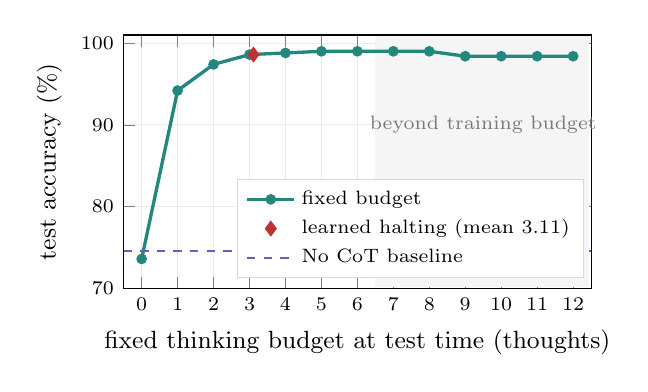
\begin{tikzpicture}
\begin{axis}[
  width=0.62\linewidth, height=4.8cm,
  xmin=-0.5, xmax=12.5, ymin=70, ymax=101,
  xlabel={fixed thinking budget at test time (thoughts)},
  ylabel={test accuracy (\%)},
  xtick={0,1,2,3,4,5,6,7,8,9,10,11,12},
  legend style={font=\scriptsize,at={(0.985,0.04)},anchor=south east,draw=black!15,fill=white,cells={anchor=west}},
  tick label style={font=\scriptsize}, label style={font=\small},
  grid=major, grid style={black!8}, clip=false]
  \fill[black!4] (axis cs:6.5,70.15) rectangle (axis cs:12.45,100.85);
  \node[font=\scriptsize,text=softgray] at (axis cs:9.5,90) {beyond training budget};
  \addplot[addteal!90!black,very thick,mark=*,mark size=1.3pt] coordinates {
    (0,73.6) (1,94.2) (2,97.4) (3,98.6) (4,98.8) (5,99.0) (6,99.0) (7,99.0) (8,99.0) (9,98.4) (10,98.4) (11,98.4) (12,98.4)};
  \addplot[only marks,mark=diamond*,mark size=2.6pt,lossred] coordinates {(3.11,98.6)};
  \addplot[mambapurple,thick,dashed,domain=-0.5:12.5,samples=2] {74.6};
  \legend{fixed budget, learned halting (mean 3.11), No CoT baseline}
\end{axis}
\end{tikzpicture}
\caption{Test accuracy of the halting-stage checkpoint when the number of thoughts is fixed at test time. Training used at most 6 thoughts.}
\label{fig:sweep}
\end{figure}

\paragraph{One thought does most of the work, and the budget extrapolates.} Figure~\ref{fig:sweep} fixes the number of thoughts at test time. A single thought lifts accuracy from 73.6\% to 94.2\%, two reach 97.4\%, and accuracy saturates at 99.0\% from five thoughts on. Budgets above the six used in training lose at most 0.6 points up to twelve thoughts. During the curriculum, accuracy rose only once three or more steps were latent, yet at test time one thought already recovers most of the gain. The halting stage trains the answer after every number of thoughts from 1 to 6 at once, and it lifted validation accuracy from 97.0\% to 99.3\% within one epoch, so it may also teach the model to compress its search into fewer steps. We did not evaluate the pre-halting checkpoint at small budgets, so we cannot yet separate the two effects.

\paragraph{Learned halting finds the knee of the curve but adapts only weakly.} The halting head stops after 3.11 thoughts on average and scores 98.6\%, half the thoughts of the fixed mode for 0.4 points (two questions). A fixed budget of three scores the same 98.6\%, so on this task the learned rule matches, but does not beat, a well-chosen fixed budget; its value is that it finds this budget without a sweep. Its thought count rises only slightly with difficulty, from 2.99 on three-step questions to 3.42 on six-step ones (Table~\ref{tab:bysteps}). The convergence rule never fired at tolerance $10^{-2}$ and always used all six thoughts: consecutive thoughts keep changing by more than 1\%, so the trajectory does not settle to a fixed point within the training budget.

\paragraph{Cost.} The two baselines took about 44 and 41 minutes on one H100 NVL, including validation, and the full 55-epoch latent run took 14.0 hours. Each thought is one more sequential pass through all 24 layers, so throughput falls as the curriculum adds thoughts (Table~\ref{tab:speed}): from 1.06 batches per second at stage 0 to 0.50 at six thoughts, roughly 0.18 seconds per thought per batch of 32. The thought steps process one token per example and are cheap in arithmetic; we attribute most of their cost to per-layer kernel launches, which a fused single-step kernel or CUDA graphs would reduce.

\begin{table}[t]
\centering
\small
\begin{tabular}{@{}lccccccccc@{}}
\toprule
Stage & 0 & 1 & 2 & 3 & 4 & 5 & 6 & final & halting \\
Thoughts & 0 & 1 & 2 & 3 & 4 & 5 & 6 & 6 & 6 (scored 1--6) \\
\midrule
Batches / s (batch 32) & 1.06 & 0.92 & 0.82 & 0.71 & 0.59 & 0.57 & 0.50 & 0.53 & 0.55 \\
\bottomrule
\end{tabular}
\caption{Training throughput by stage for Mamba-2 130M on one H100 NVL, with activation checkpointing.}
\label{tab:speed}
\end{table}

\subsection{Inference memory and latency}
\label{sec:bench}

We measure both architectures at equal size on the same H100 NVL: Mamba-2 130M and GPT-2 124M, batch 1, a 512-token prompt, bf16 weights, and $n$ thoughts followed by one answer token (Table~\ref{tab:bench}). Weights are random, which does not affect memory or time. State size is read from the cache objects, peak memory is the maximum allocated above the weights during generation, and latency is the median of repeated runs.

\begin{table}[t]
\centering
\small
\begin{tabular}{@{}llrrrrrrr@{}}
\toprule
& Thoughts $n$ & 0 & 16 & 64 & 256 & 480 & 1{,}024 & 4{,}096 \\
\midrule
\multirow{2}{*}{State / KV cache (MiB)} & Latent Mamba & 18.2 & 18.2 & 18.2 & 18.2 & 18.2 & 18.2 & 18.2 \\
& GPT-2 & 18.0 & 18.6 & 20.3 & 27.0 & 34.9 & -- & -- \\
\midrule
\multirow{2}{*}{Peak extra memory (MiB)} & Latent Mamba & 154 & 154 & 154 & 154 & 154 & 154 & 154 \\
& GPT-2 & 34.6 & 34.6 & 34.6 & 38.7 & 38.7 & -- & -- \\
\midrule
\multirow{2}{*}{Latency (s)} & Latent Mamba & 0.07 & 0.41 & 1.40 & 5.89 & 10.20 & 20.19 & 55.91 \\
& GPT-2 & 0.01 & 0.11 & 0.44 & 1.64 & 1.85 & -- & -- \\
\bottomrule
\end{tabular}
\caption{Inference after a 512-token prompt on one H100 NVL (batch 1, bf16), using the reference PyTorch implementation for Mamba. ``--'': beyond GPT-2's 1{,}024-position context.}
\label{tab:bench}
\end{table}

\paragraph{The state is constant.} Latent Mamba's state stays at 18.2\,MiB from zero to 4{,}096 thoughts. This is twice the 9.25\,MiB computed from Equation~\eqref{eq:mem} because the implementation keeps the SSM state in float32 (Section~\ref{sec:scale}); only the convolution window is bf16. GPT-2's cache grows by 36\,KiB per token and passes the Mamba state after about seven thoughts. At 480 thoughts it is $1.9\times$ larger, and GPT-2 cannot think beyond its 1{,}024-position context at all.

\paragraph{Peak memory and speed favour GPT-2 at this scale.} Peak memory above the weights is 154\,MiB for Latent Mamba at every budget, against 35--39\,MiB for GPT-2. The peak is set by the 512-token prefill, where the reference chunked scan materialises float32 intermediates, not by thinking. Latent Mamba is also 3--5$\times$ slower, about 14--21\,ms per thought against 4--6\,ms for GPT-2. Three factors contribute: Mamba-2 130M has 24 layers to GPT-2's 12; each thought runs our unfused single-step recurrence as several small PyTorch kernels per layer; and the benchmark did not use the fused \texttt{mamba\_ssm} kernels. Constant memory is therefore established, but a wall-clock advantage would need a fused single-step kernel or CUDA graphs, and reasoning much longer than ProsQA's: at six thoughts, the KV cache a Transformer adds is negligible.

\subsection{What remains}
\label{sec:remaining}

Four comparisons are still missing: Coconut with GPT-2 124M trained in the same pipeline, which isolates the backbone; a pause-token model trained through the same curriculum with empty thoughts, which separates thought content from extra computation as a trained rather than test-time control; a no-CoT model trained for 55 epochs, which matches training length; and more seeds and model sizes, together with ProntoQA and GSM8k. The released pipeline already trains the GPT-2 baseline and runs GSM8k.

% =========================================================================
\section{Discussion: why does latent reasoning help here?}
\label{sec:discussion}
% =========================================================================

The thought ablations of Table~\ref{tab:test} show that the content of the thoughts matters. Why it helps on this task is less certain; the following explanations are hypotheses.

\paragraph{Search without committing.} A written chain must choose one node of the graph per sentence. A continuous thought is a vector and can represent several candidate nodes at once, narrowing them over successive thoughts, which resembles breadth-first search. Coconut observed exactly this in GPT-2 on ProsQA by decoding thoughts through the language-model head~\cite{hao2024coconut}. The shape of our curve supports the same reading: little changes while only one or two steps are latent, and accuracy rises once three or more consecutive steps can stay in latent space, where keeping alternatives alive pays off.

\paragraph{Depth on demand.} Each thought runs the full nonlinear stack once more, so six thoughts add 144 layers of computation on top of the prompt pass. Within a single pass, Mamba's state update is linear (Equation~\eqref{eq:ssm}); the thought loop supplies the nonlinear depth that path-finding needs.

\paragraph{A large fixed-size workspace.} The 130M model carries a $24 \times 64 \times 128$ state in each of 24 layers. Thoughts read the graph facts held in this state and refine them in place, and nothing accumulates, which suits a task whose input is large (hundreds of tokens of facts) and whose reasoning is short.

\paragraph{Alternative explanations.} Three confounds were open; the test results settle one and narrow another. (i) Training length: the latent model trained for 55 epochs and the baselines for 5. No CoT peaked at its first epoch and declined afterwards, which makes ``more training'' a weak explanation, but only the 55-epoch control settles it. (ii) Extra computation: zero and noise thoughts at test time recover at most 3 of the 25 points (Table~\ref{tab:test}), so extra passes are not sufficient for a model trained with informative thoughts. Whether a model trained with pause tokens could learn to use them is still open~\cite{goyal2024pause,pfau2024dots}. (iii) Checkpoint selection: test accuracy confirms the validation result for Latent Mamba, and the baselines fall further on test, so selection does not explain the gap.

% =========================================================================
\section{Related work}
% =========================================================================

\paragraph{Latent reasoning.} Coconut~\cite{hao2024coconut} introduced continuous thoughts and observed breadth-first-search-like behaviour. Implicit CoT~\cite{deng2024icot} internalises reasoning steps through a curriculum. Pause tokens~\cite{goyal2024pause} and filler tokens~\cite{pfau2024dots} add compute without content; Pfau et al.\ show that such tokens can still carry hidden computation, which is why our zero-thought ablation is an informative control rather than a trivial one. Zhu et al.~\cite{zhu2025survey} survey the area and distinguish vertical from horizontal recurrence.

\paragraph{Recurrent depth.} Universal Transformers~\cite{dehghani2019universal} share one block across depth with ACT halting, deep equilibrium models~\cite{bai2019deq} run a layer to a fixed point, and recurrent networks trained on easy instances can extrapolate to harder ones by iterating longer~\cite{schwarzschild2021easyhard}. Geiping et al.~\cite{geiping2025recurrent} train a depth-recurrent Transformer with randomly sampled iteration counts and obtain zero-shot per-token adaptive exit. RD-VLA~\cite{tur2026rdvla} stops when the latent state converges. SST V2~\cite{aviss2026sst} streams a latent state across positions in a Transformer and deliberates per position. Wang and Reid~\cite{wang2026trmmamba} place Mamba-2 hybrid blocks inside a tiny recursive reasoning model~\cite{jolicoeur2025trm}. They leave open whether the recursion can be folded into the SSM's own state updates; Proposition~\ref{prop:collapse} and Latent Mamba give one such folding.

\paragraph{Adaptive computation and SSM expressivity.} We use ACT~\cite{graves2016act} and PonderNet~\cite{banino2021pondernet} directly. Diagonal SSMs with positive decay cannot track some states in a single pass~\cite{merrill2024illusion}; allowing negative eigenvalues helps~\cite{grazzi2025negative}. Thought steps offer a complementary route: more nonlinear passes rather than a richer transition.

\paragraph{Hybrid models.} Hybrid architectures interleave attention with Mamba layers to restore exact recall~\cite{lieber2024jamba,waleffe2024mambastudy}. Latent Mamba is compatible with them: thoughts can update the SSM layers while being kept out of the attention layers' KV cache, so memory stays constant in the thinking budget.

\paragraph{Benchmarks.} Besides ProsQA we prepare ProntoQA~\cite{saparov2023prontoqa}, a deduction benchmark over fictional ontologies, and GSM8k~\cite{cobbe2021gsm8k} in the augmented form of implicit CoT~\cite{deng2024icot}, following Coconut's settings.

% =========================================================================
\section{Limitations}
% =========================================================================

\textbf{Narrow evidence:} one synthetic dataset, one seed and one model size. Test graphs are new but share the training distribution, and ProsQA is close to saturated, so it cannot separate strong methods; the controls of Section~\ref{sec:remaining} are missing. \textbf{Halting:} the learned head matches a fixed budget of three but adapts little to difficulty, and the convergence rule never fires; ProsQA's narrow range of difficulty (3 to 6 steps) may be part of the reason. \textbf{Speed:} each thought depends on the previous output, so thoughts cannot use the parallel scan. Training throughput halves at six thoughts, and the reference implementation decodes thoughts 3--5$\times$ slower than GPT-2. Parallel training of nonlinear recurrences~\cite{aviss2026sst} and fused single-step kernels may help. \textbf{Fixed-size memory cuts both ways:} thinking cannot restore prompt details the state has already lost, so recall-heavy tasks may need hybrid attention layers, with thoughts kept out of their KV cache. \textbf{Interpretability:} thoughts are not text, and decoding them through $W$ is only a probe.

% =========================================================================
\section{Conclusion}
% =========================================================================

In a selective SSM, extra depth with a shared state is the same thing as extra time. Latent Mamba uses this to let a Mamba-2 model think in continuous space for as long as each input requires, at constant memory and with well under 1\% more parameters. Thoughts reuse the backbone unchanged, so the method needs no new kernels, trains from public pretrained checkpoints, and scores every thinking budget in one batched pass during halting training, which a growing KV cache would make expensive.

The experiment supports the idea on held-out data. On ProsQA, a pretrained 130M Mamba-2 fine-tuned with the curriculum answers 99.0\% of test questions while reasoning entirely in latent space, against 70.8\% when the same model writes its reasoning and 74.6\% when it answers directly, and in the range Coconut reports for GPT-2. The thoughts carry the reasoning: with their content zeroed or replaced by noise, accuracy falls to 76--77\%, close to answering without thoughts. A single thought already recovers most of the gain, accuracy saturates at five, and twice the training budget costs under a point. The learned halting head stops after about three thoughts at almost no loss of accuracy, halving inference compute. On GPU, the state stayed at 18.2\,MiB for budgets up to 4{,}096 thoughts, a length GPT-2 cannot reach.

The results also mark the limits of the current evidence. Halting finds a good budget but matches a fixed budget of three rather than adapting strongly to each question. At this scale and reasoning length, the reference implementation is slower than a Transformer and uses more peak memory, so the constant-memory advantage is structural rather than yet practical. Everything rests on one seed of one synthetic task. The next steps are the matched Coconut GPT-2 baseline; trained pause-token and training-length controls; more seeds and model sizes; a fused single-step kernel; tasks with long reasoning, where a constant-size state should matter most; and ProntoQA and the harder GSM8k benchmark, where Coconut trailed written chain-of-thought and Latent Mamba faces its most demanding test.

% =========================================================================
\begin{thebibliography}{99}
\setlength{\itemsep}{2pt}

\bibitem{ainslie2023gqa} J.~Ainslie, J.~Lee-Thorp, M.~de~Jong, Y.~Zemlyanskiy, F.~Lebr\'on, S.~Sanghai. GQA: Training generalized multi-query transformer models from multi-head checkpoints. EMNLP, 2023.
\bibitem{aviss2026sst} T.~Aviss. State Stream Transformer (SST) V2: Parallel training of nonlinear recurrence for latent space reasoning. arXiv:2605.00206, 2026.
\bibitem{bai2019deq} S.~Bai, J.~Z.~Kolter, V.~Koltun. Deep equilibrium models. NeurIPS, 2019.
\bibitem{banino2021pondernet} A.~Banino, J.~Balaguer, C.~Blundell. PonderNet: Learning to ponder. arXiv:2107.05407, 2021.
\bibitem{black2022neox} S.~Black, S.~Biderman, E.~Hallahan, et al. GPT-NeoX-20B: An open-source autoregressive language model. Proceedings of BigScience Episode \#5, Workshop on Challenges \& Perspectives in Creating Large Language Models, 2022.
\bibitem{blelloch1990prefix} G.~E.~Blelloch. Prefix sums and their applications. Technical report CMU-CS-90-190, Carnegie Mellon University, 1990.
\bibitem{chen2016checkpoint} T.~Chen, B.~Xu, C.~Zhang, C.~Guestrin. Training deep nets with sublinear memory cost. arXiv:1604.06174, 2016.
\bibitem{cobbe2021gsm8k} K.~Cobbe, V.~Kosaraju, M.~Bavarian, et al. Training verifiers to solve math word problems. arXiv:2110.14168, 2021.
\bibitem{dao2024ssd} T.~Dao, A.~Gu. Transformers are SSMs: Generalized models and efficient algorithms through structured state space duality. ICML, 2024.
\bibitem{dehghani2019universal} M.~Dehghani, S.~Gouws, O.~Vinyals, J.~Uszkoreit, \L.~Kaiser. Universal transformers. ICLR, 2019.
\bibitem{deng2024icot} Y.~Deng, Y.~Choi, S.~Shieber. From explicit CoT to implicit CoT: Learning to internalize CoT step by step. arXiv:2405.14838, 2024.
\bibitem{gao2020pile} L.~Gao, S.~Biderman, S.~Black, et al. The Pile: An 800GB dataset of diverse text for language modeling. arXiv:2101.00027, 2020.
\bibitem{geiping2025recurrent} J.~Geiping, S.~McLeish, N.~Jain, et al. Scaling up test-time compute with latent reasoning: A recurrent depth approach. NeurIPS, 2025.
\bibitem{goyal2024pause} S.~Goyal, Z.~Ji, A.~S.~Rawat, et al. Think before you speak: Training language models with pause tokens. ICLR, 2024.
\bibitem{graves2016act} A.~Graves. Adaptive computation time for recurrent neural networks. arXiv:1603.08983, 2016.
\bibitem{grazzi2025negative} R.~Grazzi, J.~Siems, A.~Zela, et al. Unlocking state-tracking in linear RNNs through negative eigenvalues. ICLR, 2025.
\bibitem{gu2022s4} A.~Gu, K.~Goel, C.~R\'e. Efficiently modeling long sequences with structured state spaces. ICLR, 2022.
\bibitem{gu2023mamba} A.~Gu, T.~Dao. Mamba: Linear-time sequence modeling with selective state spaces. arXiv:2312.00752, 2023.
\bibitem{hao2024coconut} S.~Hao, S.~Sukhbaatar, D.~Su, et al. Training large language models to reason in a continuous latent space. arXiv:2412.06769, 2024.
\bibitem{jolicoeur2025trm} A.~Jolicoeur-Martineau. Less is more: Recursive reasoning with tiny networks. arXiv preprint, 2025.
\bibitem{kojima2022zeroshot} T.~Kojima, S.~S.~Gu, M.~Reid, Y.~Matsuo, Y.~Iwasawa. Large language models are zero-shot reasoners. NeurIPS, 2022.
\bibitem{lieber2024jamba} O.~Lieber, B.~Lenz, H.~Bata, et al. Jamba: A hybrid Transformer-Mamba language model. arXiv:2403.19887, 2024.
\bibitem{loshchilov2019adamw} I.~Loshchilov, F.~Hutter. Decoupled weight decay regularization. ICLR, 2019.
\bibitem{martin2018parallelizing} E.~Martin, C.~Cundy. Parallelizing linear recurrent neural nets over sequence length. ICLR, 2018.
\bibitem{merrill2024illusion} W.~Merrill, J.~Petty, A.~Sabharwal. The illusion of state in state-space models. ICML, 2024.
\bibitem{micikevicius2018mixed} P.~Micikevicius, S.~Narang, J.~Alben, et al. Mixed precision training. ICLR, 2018.
\bibitem{nye2021scratchpad} M.~Nye, A.~J.~Andreassen, G.~Gur-Ari, et al. Show your work: Scratchpads for intermediate computation with language models. arXiv:2112.00114, 2021.
\bibitem{pfau2024dots} J.~Pfau, W.~Merrill, S.~R.~Bowman. Let's think dot by dot: Hidden computation in transformer language models. arXiv:2404.15758, 2024.
\bibitem{radford2019gpt2} A.~Radford, J.~Wu, R.~Child, D.~Luan, D.~Amodei, I.~Sutskever. Language models are unsupervised multitask learners. OpenAI technical report, 2019.
\bibitem{saparov2023prontoqa} A.~Saparov, H.~He. Language models are greedy reasoners: A systematic formal analysis of chain-of-thought. ICLR, 2023.
\bibitem{schwarzschild2021easyhard} A.~Schwarzschild, E.~Borgnia, A.~Gupta, F.~Huang, U.~Vishkin, M.~Goldblum, T.~Goldstein. Can you learn an algorithm? Generalizing from easy to hard problems with recurrent networks. NeurIPS, 2021.
\bibitem{shazeer2019mqa} N.~Shazeer. Fast transformer decoding: One write-head is all you need. arXiv:1911.02150, 2019.
\bibitem{tur2026rdvla} Y.~Tur, et al. Recurrent-Depth VLA: Implicit test-time compute scaling of VLA models via latent iterative reasoning. arXiv:2602.07845, 2026.
\bibitem{vaswani2017attention} A.~Vaswani, N.~Shazeer, N.~Parmar, et al. Attention is all you need. NeurIPS, 2017.
\bibitem{waleffe2024mambastudy} R.~Waleffe, W.~Byeon, D.~Riach, et al. An empirical study of Mamba-based language models. arXiv:2406.07887, 2024.
\bibitem{wang2026trmmamba} W.~Wang, F.~Reid. Tiny recursive reasoning with Mamba-2 attention hybrid. arXiv:2602.12078, 2026.
\bibitem{wei2022cot} J.~Wei, X.~Wang, D.~Schuurmans, et al. Chain-of-thought prompting elicits reasoning in large language models. NeurIPS, 2022.
\bibitem{zhang2019rmsnorm} B.~Zhang, R.~Sennrich. Root mean square layer normalization. NeurIPS, 2019.
\bibitem{zhu2025survey} R.-J.~Zhu, et al. A survey on latent reasoning. arXiv:2507.06203, 2025.
\end{thebibliography}

\end{document}
